\documentclass[border=6pt]{standalone}
\usepackage{tikz}
\usetikzlibrary{arrows.meta,calc,positioning}
\begin{document}
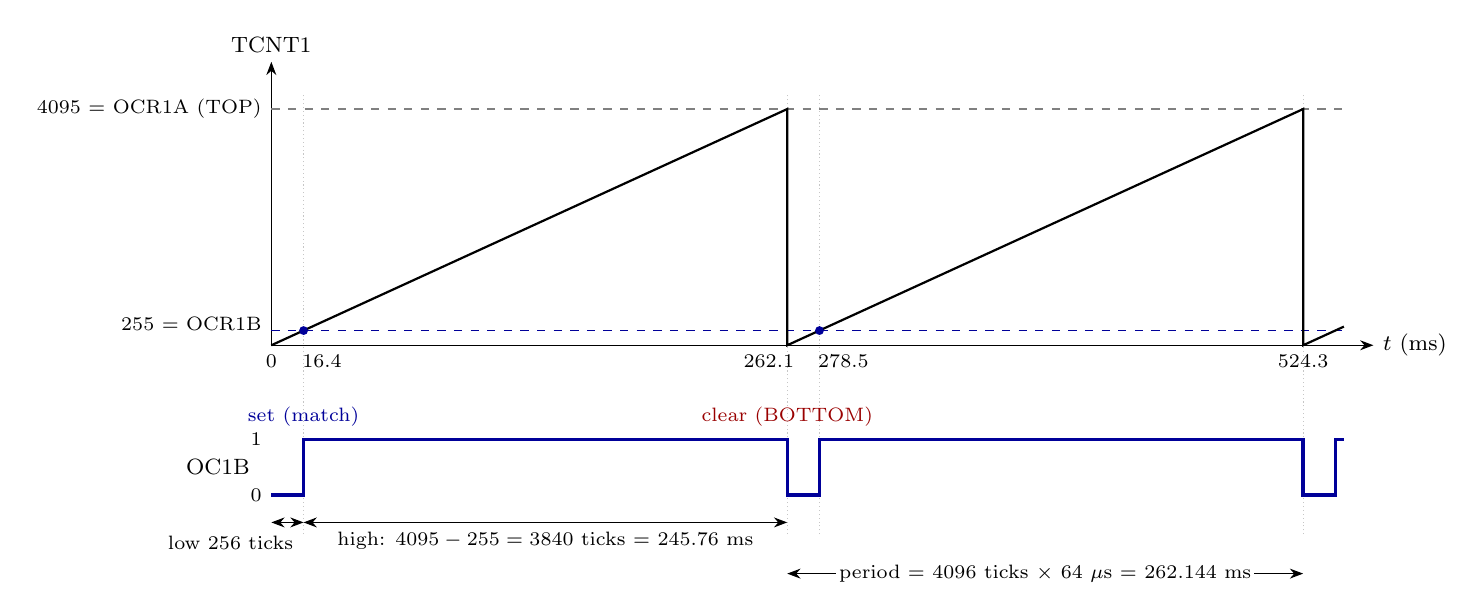
\begin{tikzpicture}[>=Stealth,font=\small,x=0.025cm,y=1cm]
% 1 unit = 1 ms. 1 tick = 64 us (1 MHz / 64). Period = 4096 ticks = 262.144 ms.
% OCR1B match at TCNT1 = 255: OC1B low for 256 ticks = 16.384 ms, high for 3840 ticks = 245.76 ms.
\def\H{3.0}% TOP = 4095
\def\C{0.1868}% 255 to scale: 3.0*255/4095
\foreach \t in {16.384,262.144,278.528,524.288} \draw[gray!45,densely dotted] (\t,-2.4) -- (\t,\H+0.2);
\draw[->] (0,0) -- (0,\H+0.6) node[above,font=\footnotesize]{TCNT1};
\draw[->] (0,0) -- (560,0) node[right,font=\footnotesize]{$t$ (ms)};
\node[anchor=east,font=\scriptsize] at (0,\H) {4095 = OCR1A (TOP)};
\node[anchor=east,font=\scriptsize] at (0,\C+0.08) {255 = OCR1B};
\draw[gray,dashed] (0,\H) -- (545,\H);
\draw[blue!60!black,dashed] (0,\C) -- (545,\C);
\draw[thick] (0,0) -- (262.144,\H) -- (262.144,0) -- (524.288,\H) -- (524.288,0) -- (545,{\H*20.712/262.144});
\foreach \t in {16.384,278.528} \fill[blue!60!black] (\t,\C) circle (1.6pt);
\node[below,font=\scriptsize] at (0,0) {0};
\node[below left=0pt and -6pt,font=\scriptsize] at (262.144,0) {262.1};
\node[below,font=\scriptsize] at (524.288,0) {524.3};
\node[below right=0pt and -4pt,font=\scriptsize] at (16.384,0) {16.4};
\node[below right=0pt and -4pt,font=\scriptsize] at (278.528,0) {278.5};
% OC1B
\begin{scope}[yshift=-1.9cm]
\node[anchor=east,font=\footnotesize] at (-6,0.35) {OC1B};
\node[anchor=east,font=\scriptsize] at (0,0.7) {1};
\node[anchor=east,font=\scriptsize] at (0,0) {0};
\draw[very thick,blue!60!black] (0,0) -- (16.384,0) -- (16.384,0.7) -- (262.144,0.7) -- (262.144,0) -- (278.528,0) -- (278.528,0.7) -- (524.288,0.7) -- (524.288,0) -- (540.672,0) -- (540.672,0.7) -- (545,0.7);
\node[font=\scriptsize,blue!60!black,anchor=south] at (16.384,0.75) {set (match)};
\node[font=\scriptsize,red!60!black,anchor=south] at (262.144,0.75) {clear (BOTTOM)};
\draw[<->] (16.384,-0.35) -- (262.144,-0.35) node[midway,below,font=\scriptsize]{high: $4095-255 = 3840$ ticks = 245.76 ms};
\draw[<->] (0,-0.35) -- (16.384,-0.35);
\node[font=\scriptsize,anchor=north east] at (16,-0.4) {low 256 ticks};
\draw[<->] (262.144,-1.0) -- (524.288,-1.0) node[midway,fill=white,font=\scriptsize,inner sep=1pt]{period = 4096 ticks $\times$ 64 $\mu$s = 262.144 ms};
\end{scope}
\end{tikzpicture}
\end{document}
